\chapter{Lo sviluppo del progetto}
\label{chap:descrizione-stage}
\noindent
In questo capitolo parlo del progetto in se e per se, analizzando il problema che mi è stato posto e come ho deciso di risolverlo.
Vado poi a fare un resoconto finale sul prodotto ottenuto e ne valuto la qualità.

\section{La metodologia e le tecnologie}
\subsection{Il metodo di lavoro}
% In questo punto parlo del metodo di lavoro che ho adottato durante l'attività di \textit{stage} per organizzare il lavoro e confrontarmi con il mi tutor.
\noindent
All'inizio della mia collaborazione con l'azienda, ho stilato, insieme al mio \textit{tutor} aziendale, un piano di lavoro per lo \textit{stage} che sarei andato a svolgere.
Tale documento contiene una suddivisione delle attività previste per ognuna delle otto settimane della mia permanenza in azienda.\\
Abbiamo deciso quindi, insieme al \textit{tutor} aziendale, che avrei seguito fedelmente questa suddivisione, organizzandomi il lavoro in modo da riuscire, ogni settimana, a completare ciò che veniva richiesto.
Le attività sono organizzate in modo da arrivare a soddisfare tutti gli obiettivi entro la fine dello \textit{stage}, tenendo conto che qualora un'attività necessiti di più tempo di quello previsto si andrà a continuarla nella settimana successiva fino a che non è finita.
Abbiamo ordinato il lavoro in modo che gli obiettivi vengano soddisfatti in base alla loro importanza, partendo quindi prima da quelli obbligatori, poi quelli desiderabili e infine i facoltativi.

\begin{figure}[H]
   \centering
   \makebox[\textwidth][c]{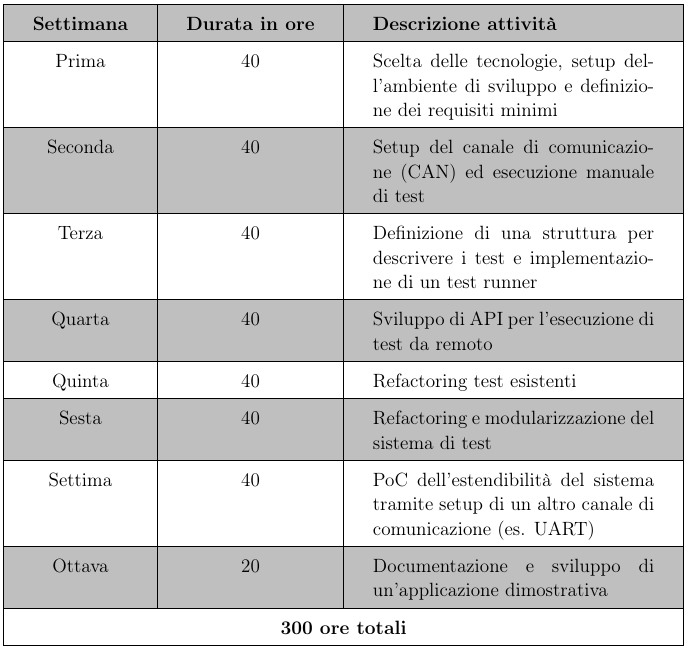
\includegraphics[width=\textwidth]{img/ripartizione_attivita.png}}
   \caption{\centering Estratto del documento "Piano di lavoro" contenente la suddivisione delle attività per ogni settimana prevista dal tirocinio.}
   \vspace{0.1cm}
   {\footnotesize Fonte: Elaborazione originale dell'autore\par}
\end{figure}

\noindent
All'inizio di ogni attività suddividevo il lavoro in più compiti atomici che avrei poi svolto durante quel periodo.
Nel particolare ho utilizzato una \textit{board} di Gitlab, all'interno della quale segnavo, e tenevo nota, di tutte le attività pianificate e le dipendenze che avevano tra di loro.
Questo mi permetteva di avere una chiara visione dell'andamento e dell'ordine in cui svolgere le attività, senza incorrere in dipendenze inaspettate che interferissero con un fluido andamento del lavoro.\\

\noindent
Alla fine di ogni settimana era previsto un resoconto (di persona) durante il quale mostravo al mio \textit{tutor} il risultato di quella settimana di lavoro, ricevevo un \textit{feedback} e gli spiegavo quali attività prevedevo di svolgere per la settimana successiva.
Oltre a questo resoconto settimanale, si aggiungevano le interazioni quotidiane con il mio \textit{tutor} nelle quali gli facevo note le difficoltà che incontravo e i progressi fatti.
Questa stretta interazione ci permetteva sia di rimanere sempre allineati sullo stato del progetto, sia di affrontare eventuali problematiche sul nascere.


\subsection{Le tecnologie utilizzate}
% In questo punto descrivo quali tecnologie e strumenti (\textit{software} e \textit{hardware}) ho utilizzato per la progettazione e sviluppo del progetto.
\noindent

\section{Analisi}
% In questa sezione spiego il problema che sono andato ad affrontare e spiego la teoria che ci sta dietro.
% Nel particolare parlo dei principali protocolli utilizzati, spingendomi nel dettaglio quanto basta perché si possa comprendere più facilmente le sezioni successive.
% Oltre a ciò spiegherò la teoria che sta dietro i \textit{test} implementati, motivando il loro scopo in relazione all'obiettivo del progetto.
\noindent

\section{Progettazione}

\subsection{Introduzione}
% Breve sezione di introduzione sull'architettura del progetto nel suo complesso.
\noindent

\subsection{Le classi `Target'}
% In questa sezione spiego come ho rappresentato i dispositivi \textit{target} sui quali verranno lanciati i controlli di sicurezza.
\noindent

\subsection{Le classi `Test'} \label{dev:classi_test}
\noindent
In questa sezione spiego come ho rappresentato i \textit{test} da lanciare, partendo dai moduli che mi sono stati forniti e sui quali ho effettuato il \textit{refactoring}.
Questa parte riprende diversi concetti di §3.3, o per meglio dire ne rappresenta l'applicazione concreta all'interno del progetto.

\subsection{Creazione ed esecuzione}
\noindent
In questa sezione spiego i servizi che si occupano della creazione e l'esecuzione delle classi di test.
La creazione comprende una classe \textit{factory} e un \textit{pattern registry}; l'esecuzione comprende un \textit{service} per l'esecuzione del singolo \textit{test} e un altro per la gestione di più \textit{test} eseguiti in serie.
In merito a quest'ultimo parlerò anche della soluzione adottata per tenere traccia del \textit{context} che permette ai \textit{test} di prendere in \textit{input} il risultato dei \textit{test} eseguiti in precedenza.

\subsection{Persistenza}
\noindent
In questa sezione spiego i servizi utilizzati per implementare uno storico dei \textit{test} che conservi anche i risultati di quest'ultimi.
Descriverò il \textit{service} addetto alla persistenza e il \textit{pattern repository} che interagisce con il \textit{database SQLite}, motivando la scelta di quest'ultimo rispetto a un tradizionale \textit{DBMS}.

\subsection{API}\label{dev:api}
\noindent
In questa sezione spiego gli \textit{endpoint} messi a disposizione dall'\textit{API} implementata per accedere ai servizi del \textit{framework}.

\subsection{\textit{Frontend} }
\noindent
In questa sezione spiego il ruolo del \textit{frontend} come applicazione dimostrativa.
È un punto un po' fuorviante, in quanto il senso del frontend è dimostrare l'estendibilità del progetto ad altre componenti che non abbiano diretto accesso alla logica interna del \textit{framework}.

\section{Programmazione}
\noindent
In questa sezione parlo della stesura del codice ed eventuali difficoltà/incoerenze rispetto alla progettazione che ho incontrato.
Parto parlando prima dello sviluppo in \textit{Python} del \textit{framwork} e successivamente mi soffermo sullo sviluppo del \textit{firmware} in \textit{C}.

\section{Verifica e validazione}
\noindent
In questa sezione parlo dei controlli effettuati per verificare la correttezza del codice.
Mi soffermo sul motivare perché si non ho puntato a un alta copertura di codice e su quali punti mi sono concentrato.

\section{Resoconto del lavoro svolto}
\subsection{I risultati conseguiti}
\noindent
In questa sezione discuto i risultati raggiunti sul piano qualitativo che su quello quantitativo, specificando i prodotti \textit{software} e di documentazione che sono risultati alla fine del progetto.
Faccio poi una presentazione del progetto completo nel suo insieme, discutendone i diversi tipi di utilizzi che se ne possono fare dal punto di vista di un utente esterno.

\subsection{Migliorie possibili}
\noindent
In questa sezione parlo di possibili migliorie che scoperto riguardando il progetto una volta finito.
Cerco di dare una mia valutazione alle componenti del prodotto in relazione all'impegno che è servito per realizzarle, ne riconosco le limitazioni, spiego su cosa mi concentrerei se dovessi continuare a lavorarci.
Discuto inoltre se vi sono scelte che farei diversamente se dovessi ricominciare da zero il progetto.
